\section*{Method-specific 1000-gene panel comparison}
We constructed six 1000-gene panels from existing method outputs: HVG, differential expression (DE; combined across Immune\_broad and Malignant\_vs\_Other contexts by best aggregated rank), SpaPROS, scGeneFit, Random Forest (RF), and the curated final panel. Gene symbols were mapped to the active AnnData var\_names; when necessary, symbol mapping from the AnnData var was used to resolve identifiers. Each panel was saved under panels/ as CSV (var\_names).

Using the active 50k-cell AnnData (with baseline UMAP computed on the 3k HVG feature space), we recomputed PCA, kNN (k=15), and UMAP for each panel (1k features), and compared the resulting embeddings to the baseline. We quantified resemblance via mean Jaccard overlap of kNN neighborhoods vs. baseline, and trustworthiness using the baseline UMAP as the reference space.

To evaluate clustering agreement, a single Leiden resolution (selected once on the HVG-1k panel to target ~\,20\% deviation from the number of unique cell types) was applied to all panels. Agreement with ground-truth labels (obs[cell\_type]) was reported using ARI and NMI, and class compactness was summarized with the Silhouette Index (SI) computed in UMAP space.

Figure~\ref{fig:panel_radar} summarizes ARI, NMI and SI across panels as a radar plot. Representative UMAP comparisons (baseline vs. panel-only) are shown in Figure~\ref{fig:panel_umap_compare}. The full metrics table is available at path: selection\_expert/panel\_comparison/metrics/panel\_metrics.csv.

\begin{figure}[h]
  \centering
  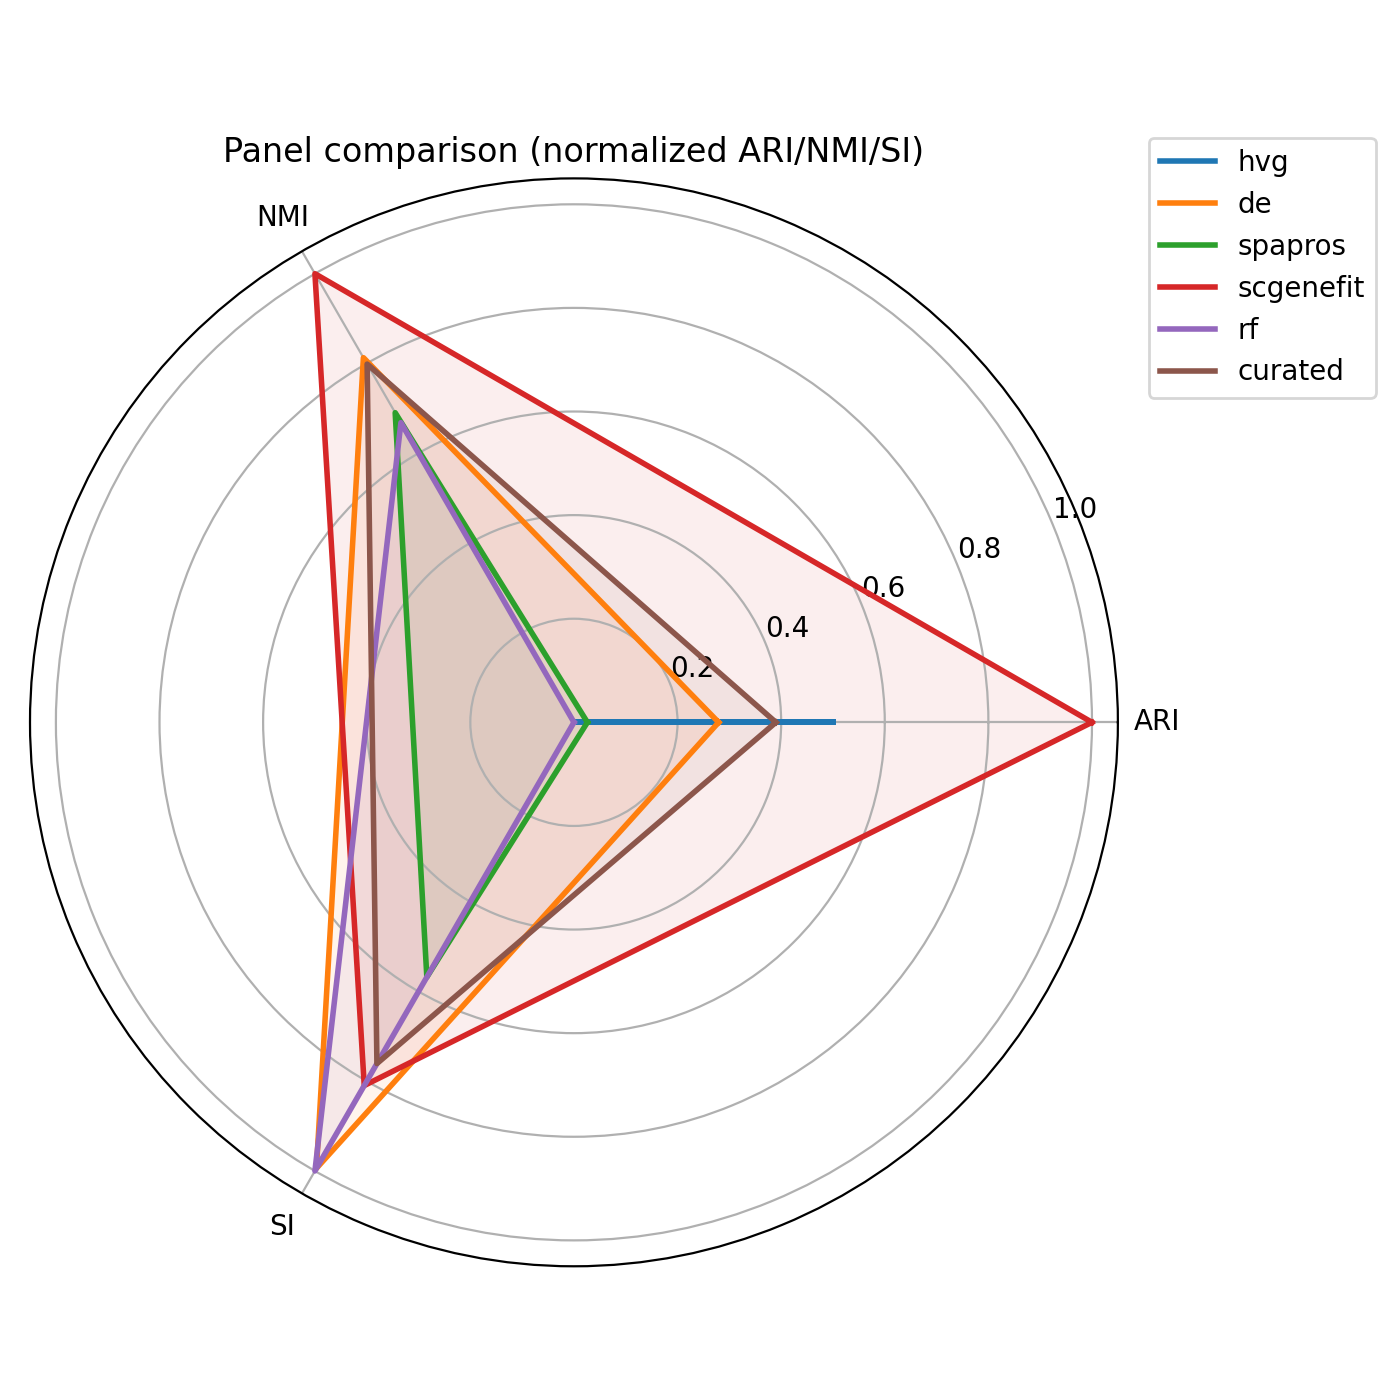
\includegraphics[width=0.55\textwidth]{selection_expert/panel_comparison/figures/panel_radar_ari_nmi_si.png}
  \caption{Radar plot of ARI, NMI, and SI across the six 1k-gene panels.}
  \label{fig:panel_radar}
\end{figure}

\begin{figure}[h]
  \centering
  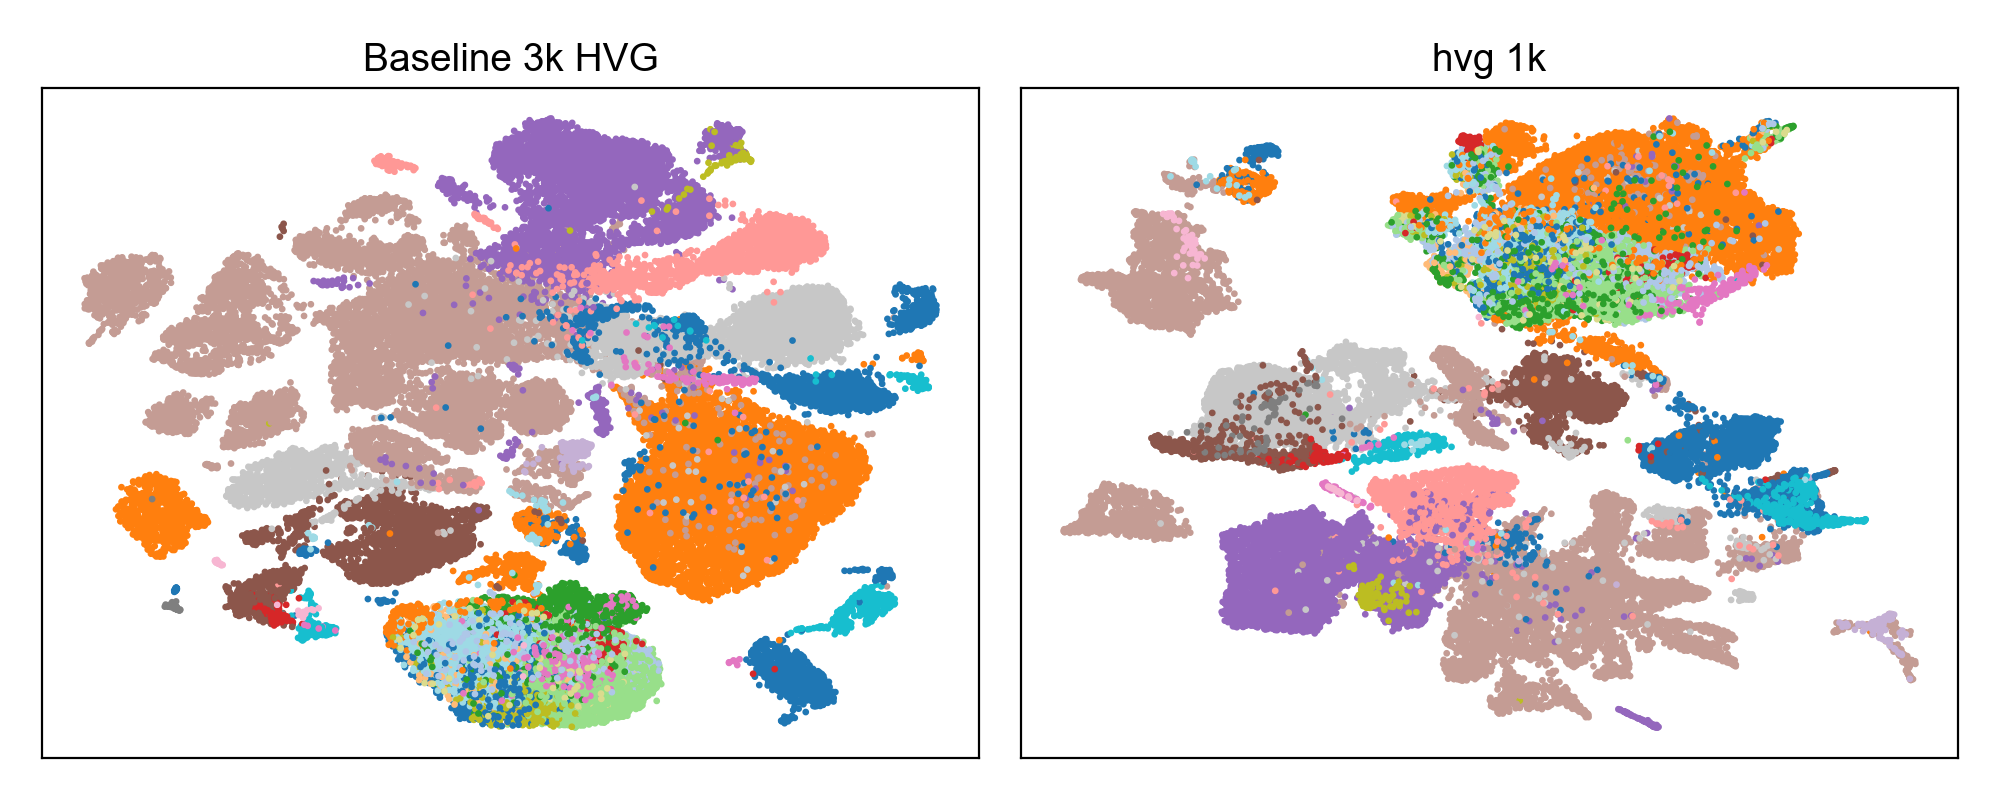
\includegraphics[width=0.95\textwidth]{selection_expert/panel_comparison/figures/umap_compare_hvg.png}
  \\
  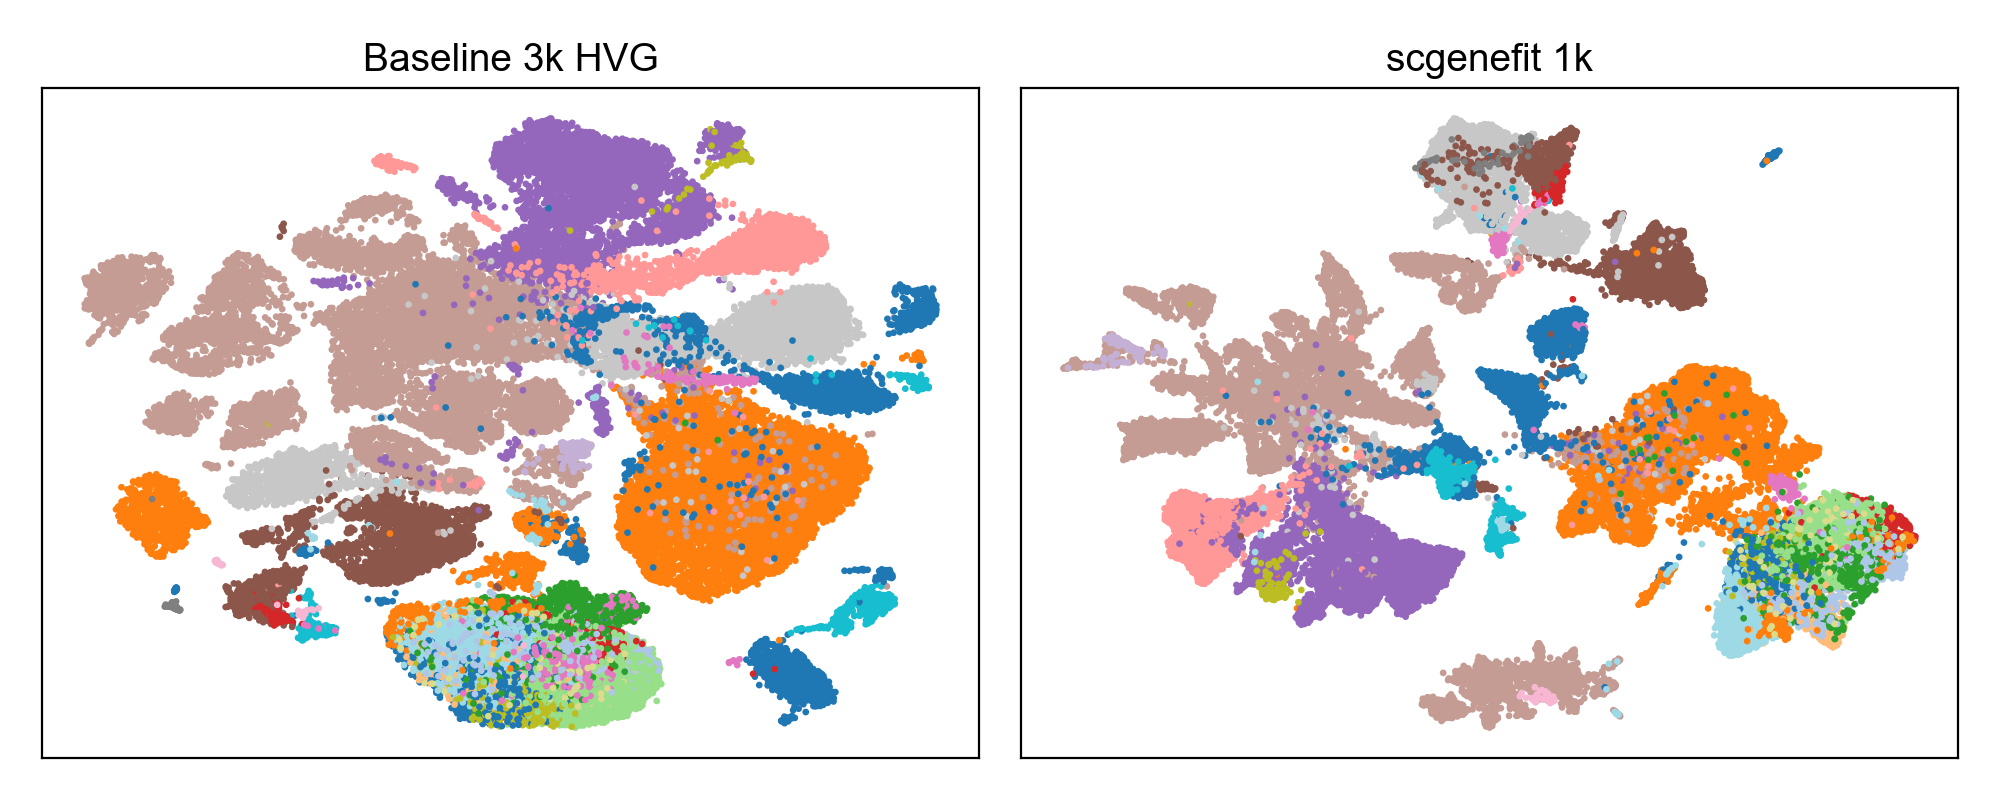
\includegraphics[width=0.95\textwidth]{selection_expert/panel_comparison/figures/umap_compare_scgenefit.png}
  \caption{UMAP comparison between baseline (left) and panel-only embeddings (right) for selected panels.}
  \label{fig:panel_umap_compare}
\end{figure}
